\def\year{2020}\relax

\documentclass[letterpaper]{article} %DO NOT CHANGE THIS
\usepackage{aaai20}  %Required
\usepackage{times}  %Required
\usepackage{helvet}  %Required
\usepackage{courier}  %Required
\usepackage{url}  %Required
\usepackage{graphicx}  %Required
\frenchspacing  %Required
\setlength{\pdfpagewidth}{8.5in}  %Required
\setlength{\pdfpageheight}{11in}  %Required
\setcounter{secnumdepth}{0}  
\usepackage{subfigure}

\begin{document}
% The file aaai.sty is the style file for AAAI Press 
% proceedings, working notes, and technical reports.
%
\title{Reinforcement Learning in Chess}
\author{Jason Chu, Stephen Li, Wei Min Loh\\
\{jjchu, s575li, wmloh\}@uwaterloo.ca\\
University of Waterloo\\
Waterloo, ON, Canada\\
}
\maketitle

%%%%%%%%%. Abstract %%%%%%%%%

\begin{abstract}
{\bf Complete this section for D4.}

The {\it Abstract} should be at most 150 words long, and should summarize briefly what your project is about.  This includes the motivation for the problem (2-3 sentences), the problem you tackled (2-3 sentences), and your main results (1-2 sentences).   
\end{abstract}

%%%%%%%%%. Introduction %%%%%%%%%

\section{Introduction} 

Chess is a deeply complicated strategy game whose complexity extends even beyond the world's best human players in the present day. With active AI chess research starting as early as the 1950s, it wasn't until 1997 that a chess AI, "Deep Blue", had claimed victory over the world chess champion for the first time. Evolution in computer chess has continued ever since; currently in 2020, new techniques in AI and machine learning have enabled chess artificial intelligence to greatly exceed human limits in ability, and human players now rely on chess engines for study and game analysis. The boundaries of chess AI are constantly being pushed, and computer chess continues to be an active realm of research today.

The methods used by many of the historical chess programs rely on search. There are an estimated $10^{43}$ legal positions in chess, and given this large number, it is very expensive to perform search for every move made. As such, it would be desirable for performant chess programs to avoid such enormous computations.

Convolutional neural networks are able to perform computations in constant time. As such, having one serving as the core of a chess program would decrease the required computation power significantly during a game when compared to earlier chess programs.

The goal of this project is to explore modern search techniques in AI and machine learning to efficiently generate a convolutional neural network which plays chess at a competitive level. Due to time and hardware constraints, emphasis is placed on search techniques with efficient pathing and pruning strategies. Performance of the network will be determined in an ELO rating system, a system which considers a player's rating based on other players of similar strength. Applying these techniques, we aim to evaluate and investigate the performance of our AI against both human and computer opponents in the real world.

%
\begin{itemize} 

\item 
{\bf For D1, describe the problem and your methodologies only.  Then, complete this part for D4. }

Describe, at a high-level, the problem you tackled and your main results.  What research questions are you trying to answer?   What methodologies did you used to answer the question? What are the performance measures that you used to evaluate the methodologies?   Describe your key findings in 2-3 sentences. (2-3 paragraphs)

\item 
{\bf Complete this bullet point for D4.}

Emphasize your contributions.  How should we interpret the results?  Why should people care about this work?   Does this project introduce any novel techniques or reveal any unexpected findings?  In bullet point forms, list 3-4 key contributions of your project.

\end{itemize}

%%%%%%%%%. Related Work %%%%%%%%%
\newpage
\section{Related Work} 

% https://www.hotchips.org/wp-content/uploads/hc_archives/hc10/2_Mon/HC10.S4/HC10.4.1.pdf
% http://www.tcm.phy.cam.ac.uk/BIG/pob24/deep_blue.pdf
Researchers have contemplated many approaches to solving chess over the years. Deep Blue, the first proven computer program to reach superhuman proficiency in chess, adopted the approach of highly-parallel search systems \cite{DeepBlue}. The major improvements from previous iterations of such system stem from algorithmic design and hardware upgrades. The evaluation function primarily works by estimating the state based on static and dynamic features. The development of search capability of Deep Blue focuses on hardware accelerations such as mounting 480 chess accelerator chips on a supercomputer. There were modifications to the minimax search, particularly using the null move pruning technique. This is accompanied by the algorithms being implemented on the circuitry level which gave Deep Blue a massive boost in parallel searches (approximately 200 million chess position searches per second). However, the approach outlined by the paper does not offer much relevant algorithmic insights since it heavily relies on chess databases.

After the defeat of Garry Kasparov by Deep Blue, a stagnation in computer chess persisted as researchers pursued different research areas \cite{deepblueshistory}. However, before the rise in popularity of deep learning, Sebastian Thrun published a pioneering paper on the application of artificial neural networks on computer chess in 1995. Prior computer chess programs utilize handcrafted features to characterize game states which may not generalize well. Thrun published the findings on adopting explanation-based neural network learning (EBNN) as a means to replace traditional evaluation functions which, albeit winning only 13\% of matches against GNU-Chess, revealed potential and caveats with neural network learning \cite{thrun}. Temporal difference learning (TD) was used in conjunction with neural network to stabilize the training process in the presence of delayed rewards. Unlike other computer chess programs, the paper does not offer a sampling technique but rather relies on a database of expert chess games.

A breakthrough in effective sampling techniques was proposed by Kocsis et al. The introduction of the Monte Carlo tree search (MCTS) enabled selective sampling which helped overcome the massive sample space of a Markov Decision Process \cite{banditmcts}. This development stems from a bandit algorithm called UCB1 that determines which internal nodes to expand, as opposed to exploring in a systematic fashion. The underlying principle of this algorithm aligns with the trade-offs posed by a MDP: exploration versus exploitation. By introducing a randomized algorithm that gradually becomes greedy in the choice of node expansion, the expanded state spaces are shown to be sufficiently wide and deep by the end of the search. Important theoretical results from the paper include convergence in expectation of expected rewards and convergence of failure probability. The experimental result compliments the theory where the UCT algorithm requires fewer samples to achieve a particular error rate when compared to competing algorithms: ARTDP and PG-ID. In general, the Monte Carlo tree search offers a valuable algorithm as a means to explore state spaces.

With the rise in deep learning methods and superior hardware resources, researchers returned to the computer chess with different toolkits. Most have already abandoned dedicated hardware approaches such as Deep Blue. Instead, the recent methods approach focuses on a data-centric way to fit the evaluation function. DeepChess is a particular design that adopted this new paradigm and harnesses these recent advancements \cite{deepchess}. Unlike previously discussed approaches, DeepChess does not rely purely on reinforcement learning and search but uses both supervised and unsupervised learning. This is possible due to the availability of vast amounts of expert chess match data. DeepChess does not work directly with the raw state representation; David et al. suggested the use of the deep belief network (DBN) to extract high level features to avoid high dimensionality and overfitting the evaluation function. The DBN is trained with 2,000,000 chess positions with 50\% White-win positions and 50\% Black-win positions.

A Siamese network was designed with the purpose of comparing which of the two given states is more likely to win the game. The DBN is stacked on the two heads with shared weights to serve as high level feature extractors while the subsequent layers evaluates the value function \cite{deepchess}. The Siamese network is trained with 1,000,000 unique positions, achieving a spectacular validation accuracy of 98.0\%. DeepChess, however, uses a relatively outdated variant of search: $\alpha$-$\beta$ search. It is used to evaluate certain positions from the root at a predefined depth. The authors recognized the issue of poor computational performance due to the massive number of pairwise state comparisons which was partially rectified with a smaller Siamese network without a significant decrease in accuracy.

The success of AlphaGo by Google DeepMind brought attention to the potential of deep reinforcement learning \cite{alphago2016} in games. AlphaZero builds upon the strengths of AlphaGo and generalizes the algorithm to solve chess, Shogi and Go. AlphaZero combines the use of deep learning (like DeepChess) with an improved general-purpose MCTS \cite{alphazero2018}. The key distinction from DeepChess is the complete lack of human guidance and hence, minimized bias in the policy. This is attributed to the use of MCTS which is a form of self-play. The MCTS samples games of self-play (generated from competing population of AlphaZero agents) and picks the best agents for subsequent iterations, which replaces the current agent if applicable. The two-head policy-value network is fundamentally similar to the Siamese network by David et al., but uses convolutional layers instead of fully connected layers. This neural network $f_\theta(s)$ outputs the policy vector and predicted outcome $(\textbf{p}, v)$ where $\textbf{p}$ is a biased estimate of the true proportion of winning state in MCTS and $v$ is an estimate of the expected outcome of the game in a given state. The training of the network from simulated data, using only the rules of the game as input, achieved superhuman intelligence in just several hours, and was deemed to be the current state-of-the-art. However, the method requires extensive computational resources and time which may be a significant hindrance to other researchers.

%%%%%%%%%. Methodology %%%%%%%%%

\section{Methodology}

{\bf Complete this section for D2.}

The {\it Methodology } section ($\sim$2 pages) describes the algorithms that you chose to implement.  Describe in details how each algorithm works.  Include their mathematical formulations, if necessary.  Include pseudo-code, if necessary.  If you had to extend an existing algorithm in order for it to work with the problem, describe in details what is different/new.  Provide a rationale for why you selected these particular algorithms and how they are appropriate for the problem.  You should provide enough details so that someone can reproduce the steps and replicate your results.  

If you are tackling a machine learning problem, you may be using an existing data set or creating a new data set.  In this case, you should describe the data-set that you are analyzing as well as any data filtering and merging procedures that you used to prepare/create your data-set.  Your description should. include the size of the data-set(s) (i.e., number of examples), whether the class labels are balanced/imbalanced, the meaning of the features, and other unique characteristics of the data-sets.   Explain why the data-sets are appropriate for your problem and what are their limitations.  Include the URL of the websites from which you downloaded the data-set(s).

You should also describe any pre-processing steps you took to prepare or create the final data-set that you used to train and test the algorithms.  Examples of pre-processing steps include procedures for joining multiple data-sets, filtering out certain examples, scaling features, etc.  Provide the rationale for why you are using these data preparation procedures, with enough details so that someone can reproduce the steps and replicate your results.   For example, if you chose to re-scale certain features, explain how the re-scaling was done and why.   


%%%%%%%%%. Example of subfigure and 2-column figure layout %%%%%%%%%

\begin{figure*}[t!]
\centering
\subfigure[image A]{
\fbox{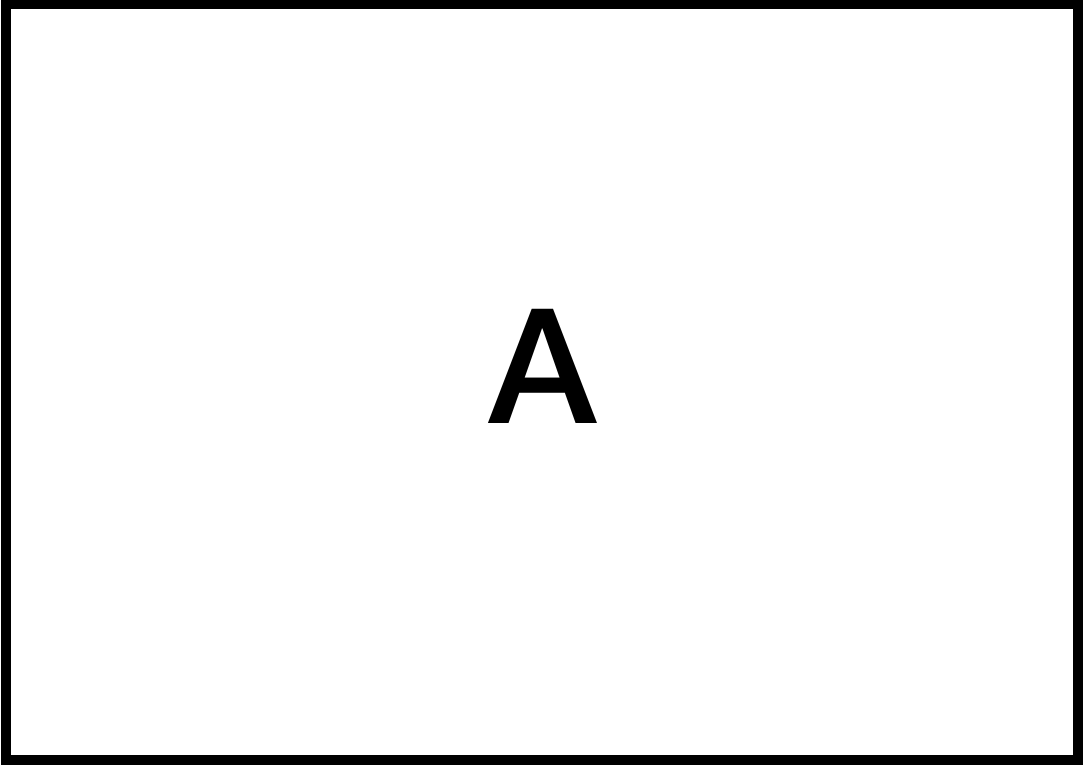
\includegraphics[height=2.6cm]{figures/A}}
\label{fig:a}
}\hfill
\subfigure[image B]{
\fbox{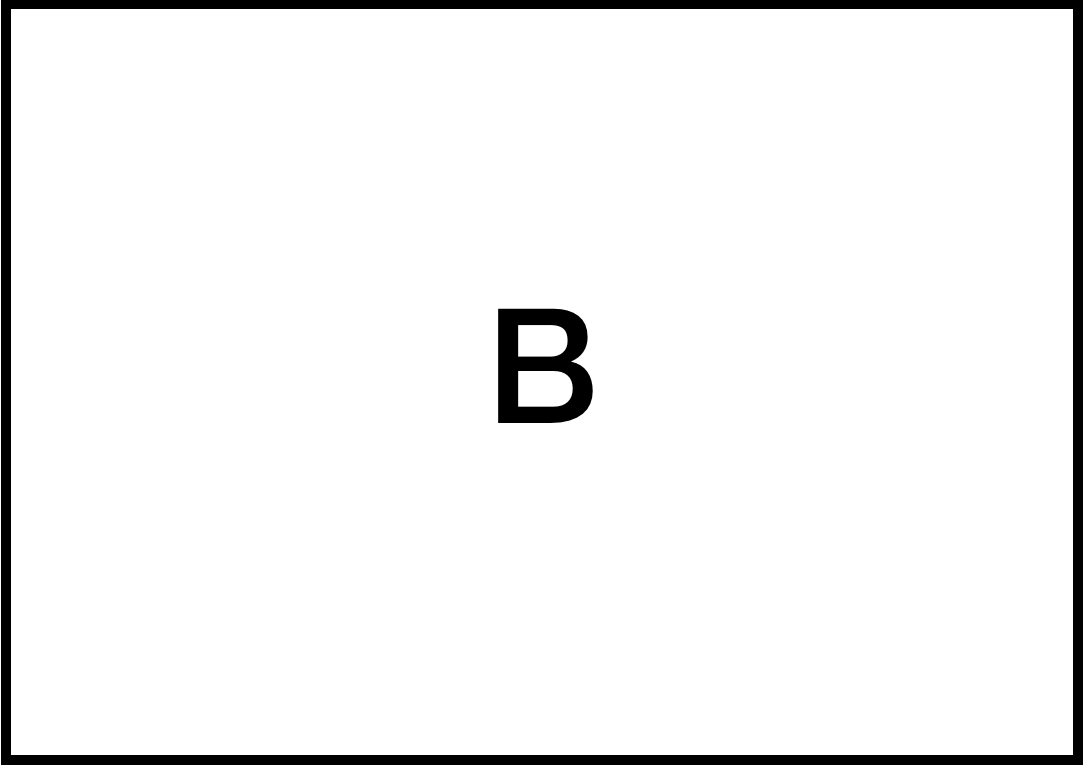
\includegraphics[height=2.6cm]{figures/B}}
\label{fig:b}
}\hfill
\subfigure[image C]{
\fbox{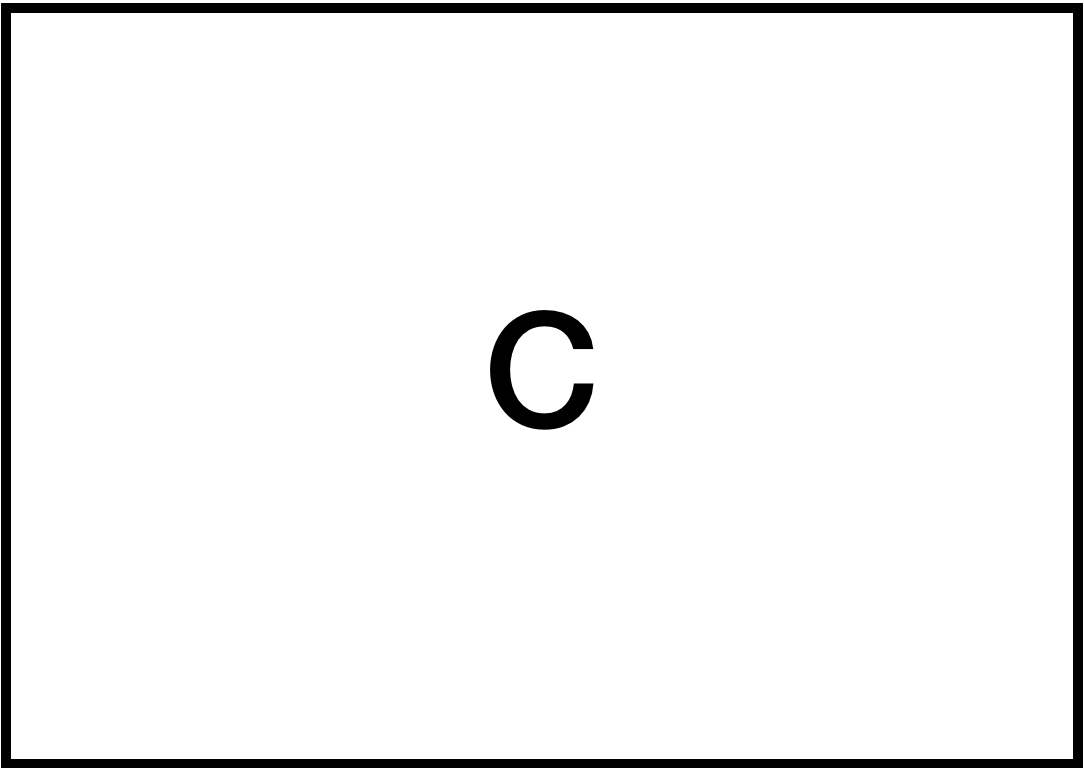
\includegraphics[height=2.6cm]{figures/C}}
\label{fig:c}
}\hfill
\subfigure[image D]{
\fbox{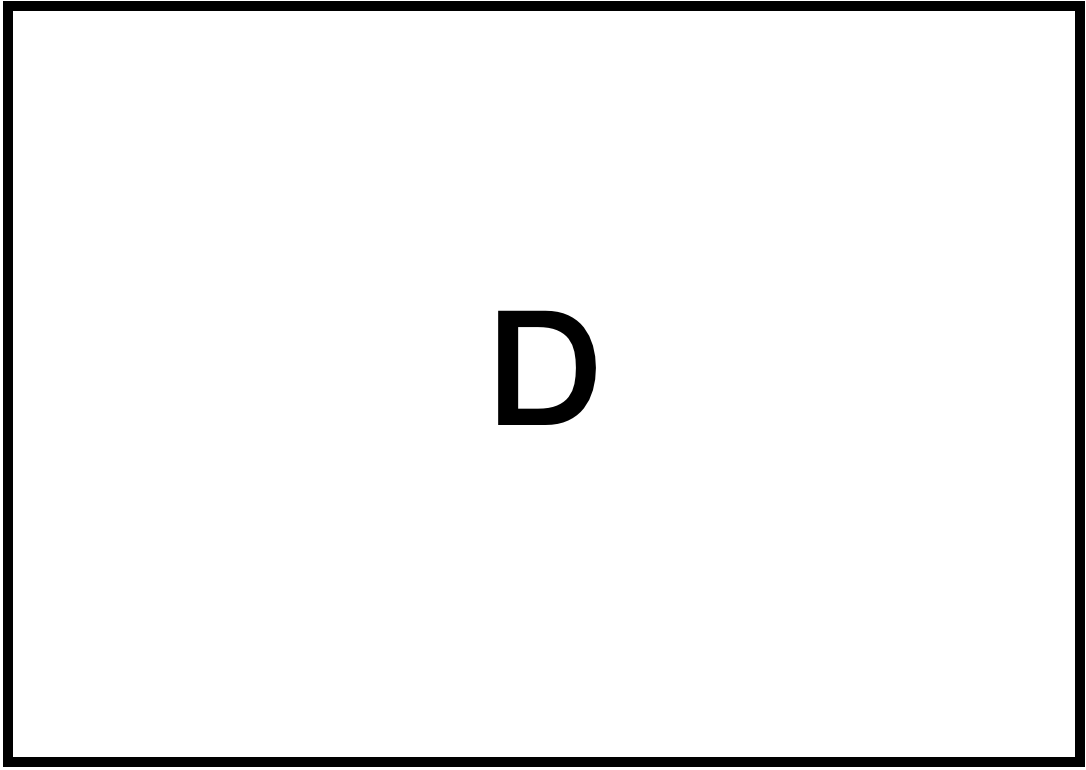
\includegraphics[height=2.6cm]{figures/D}}
\label{fig:d}
}\hfill
\caption{Another example of figure layout}
\label{fig:figures_across}
\end{figure*}

%%%%%%%%%. Results %%%%%%%%%

\section{Results}

{\bf Complete this section for D2 and D3.}

The {\it Results} section ($\sim$2 pages) describes how you evaluated the algorithms and reports the findings.  

{\bf Complete the following two paragraphs for D2.}

Describe the measures that you used to evaluate the algorithms.  Be as precise as possible by including their mathematical formulations.  Provide a rationale for why these performance metrics are appropriate for your problem.

Describe other details about your experimental design.  If you are tackling a machine learning problem, include details such as how you created the training, validation and test set, how you selected the model's hyper-parameters, etc.    

{\bf Complete the following two paragraphs for D3.}

Describe the findings from your evaluation.  Describe both (a) how well your techniques worked, and (b) what you learned about the problem through these techniques.  

Prepare figures (e.g., Figure \ref{fig:results2}) and tables (e.g., Table \ref{tab:results1}) to describe your results clearly.  Make sure to label your figures and tables and explain them in the text.  If you are comparing the performance of algorithms, include statistical tests to assess whether the differences are statistically significant.  If possible, describe how your techniques compare to prior work.  

\begin{table}[h!]
    \centering
    \normalsize{
    \begin{tabular}{ l c }
    \hline
         Techniques & F-1 Score\\
         \hline
          Baseline & 0.80 \\
          Another Baseline & 0.76\\
          My Awesome Algorithm & {\bf 0.95}\\
         \hline
    \end{tabular}}
    \caption{example of a table summarizing the results}
    \label{tab:results1}
\end{table} 

\begin{figure}[htbp!]
  \centering
  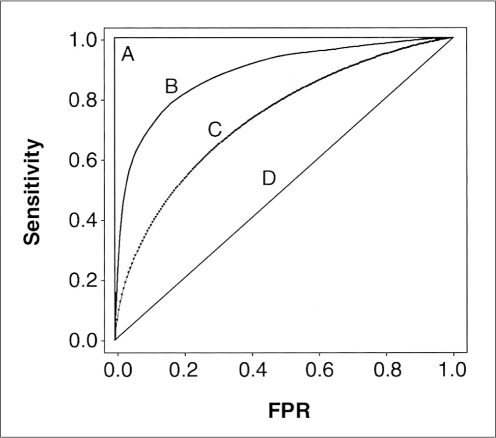
\includegraphics[width=0.9\linewidth]{figures/roc.png}
  \caption{ROC curve of my awesome algorithms}
  \label{fig:results2}
\end{figure}


%%%%%%%%%. Discussion %%%%%%%%%

\section{Discussion}

{\bf Complete this section for D4.}

The {\it Discussion} section ($\sim$1 pages) describes (a) the implications of your results, and (b) the impact and the limitations of your approach.  

For the results, describe how a reader should interpret them.  Try to form concise take-away messages for the reader.  For your approach, describe the extent to which your approach helps to solve the problem.  Describe any limitations of your approach.  If possible, compare your results and your approach to that of prior work. 

%%%%%%%%%. Conclusion %%%%%%%%%

\section{Conclusion}

{\bf Complete this section for D4.}

The {\it Conclusion} section ($\sim$0.5 pages) provides a brief summary of the entire paper.  In this section, describe 
\begin{itemize}
    \item the motivation, the problem, and your results, and
    \item 3-4 promising future directions.
\end{itemize}

%%%%%%%%% Bibliography %%%%%%%%%
\newpage
\bibliographystyle{aaai}
\bibliography{report}

\end{document}
